% Source PDF page 555 (printed p. 541)
这里假定上确界可以取得。另一方面，如果参与者2先作选择，策略便反过来，参与者1向参与者2的最终支付为
\begin{equation}\sup_v\inf_u f(u,v).\tag{10.31}\end{equation}
支付 (10.30) 总是大于或等于 (10.31)；二者之差可解释为后行动、并知道对方行动的一方所享有的优势。如果对所有 $u,v$ 都有
\[f(u^\star,v)\le f(u^\star,v^\star)\le f(u,v^\star),\]
就称 $(u^\star,v^\star)$ 是博弈的一个解，或博弈的一个鞍点。当解存在时，后行动没有优势；$f(u^\star,v^\star)$ 是支付 (10.30) 和 (10.31) 的共同值。（见习题3.14。）

若对每个 $v$，$f(u,v)$ 关于 $u$ 凸，且对每个 $u$，$f(u,v)$ 关于 $v$ 凹，称该博弈为\emph{凸凹博弈}。$f$ 可微且凸凹时，博弈的鞍点由 $\nabla f(u^\star,v^\star)=0$ 刻画。

\subsubsection*{用不可行初始点牛顿法求解}
对于收益函数二阶可微的凸凹博弈，可用不可行初始点牛顿法求解。定义残差
\[r(u,v)=\nabla f(u,v)=\begin{bmatrix}\nabla_u f(u,v)\\\nabla_v f(u,v)\end{bmatrix},\]
再应用不可行初始点牛顿法。在博弈语境中，不可行初始点牛顿法就简称为凸凹博弈的牛顿法。

若 $Dr=\nabla^2f$ 的逆有界，并在下水平集
\[S=\{(u,v)\in\dom f\mid\norm{r(u,v)}_2\le\norm{r(u^{(0)},v^{(0)})}_2\}\]
上满足 Lipschitz 条件，就能保证不可行初始点牛顿法收敛，其中 $u^{(0)},v^{(0)}$ 是参与者的初始选择。

无约束最小化中的强凸性条件，在这里有一个简单对应。若存在 $m>0$，使所有 $(u,v)\in S$ 都满足 $\nabla_{uu}^2f(u,v)\succeq mI$ 和 $\nabla_{vv}^2f(u,v)\preceq-mI$，就称收益函数为 $f$ 的博弈是\emph{强凸凹}的。不出所料，这一强凸凹假设蕴含逆有界条件，见习题10.10。

\subsection{例子}
\subsubsection*{一个简单例子}
用等式约束解析中心问题 (10.25) 说明不可行初始点牛顿法。第一个例子是随机生成的 $n=100$、$m=50$ 的实例，问题可行且有下界。采用不可行初始点牛顿法，原始与对偶初始点为 $x^{(0)}=\one$、$\nu^{(0)}=0$，回溯参数为 $\alpha=0.01$、$\beta=0.5$。

% Source PDF page 556 (printed p. 542)
图10.1分别给出原始和对偶残差范数随迭代次数的变化，图10.2给出步长。第8次迭代取完整牛顿步，因此原始残差变为几乎零，并一直保持几乎为零。大约从第9次迭代开始，对偶残差二次收敛到零。

\subsubsection*{一个不可行的例子}
再考虑一个与上例维数相同，但 $\dom f$ 与 $\{z\mid Az=b\}$ 不相交、即不可行的实例。（它违反了本章关于问题 (10.1) 可解的基本假设，也违反第10.2.4节的假设；本例只是说明，当 $\dom f$ 与 $\{z\mid Az=b\}$ 不相交时，不可行初始点牛顿法会发生什么。）图10.3给出该例的残差范数，图10.4给出步长。当然，这里步长始终达不到 $1$，残差也不收敛到零。

\subsubsection*{一个凸凹博弈}
最后的例子是 $\R^{100}\times\R^{100}$ 上的凸凹博弈，收益函数为
\begin{equation}f(u,v)=u^\T Av+b^\T u+c^\T v-\log(1-u^\T u)+\log(1-v^\T v),\tag{10.32}\end{equation}
定义域为
\[\dom f=\{(u,v)\mid u^\T u<1,\ v^\T v<1\}.\]
问题数据 $A,b,c$ 随机生成。从 $u^{(0)}=v^{(0)}=0$ 出发，采用回溯参数 $\alpha=0.01$、$\beta=0.5$ 的不可行初始点牛顿法，其进展见图10.5。

\section{实现}
\subsection{消元}
为实现消元法，必须计算满秩矩阵 $F$ 与向量 $\widehat x$，使
\[\{x\mid Ax=b\}=\{Fz+\widehat x\mid z\in\R^{n-p}\}.\]
第C.5节介绍了几种计算方法。

\subsection{求解 KKT 系统}
本节介绍计算牛顿步或不可行牛顿步的方法，两者都要求解具有 KKT 形式的一组线性方程。

% Source PDF page 557 (printed p. 543)
\begin{figure}[htbp]\centering
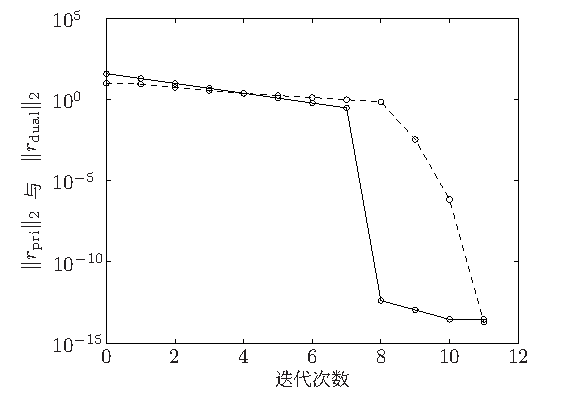
\includegraphics[width=.72\textwidth]{ch10-01.pdf}
\caption*{图10.1\quad 不可行初始点牛顿法求解具有100个变量、50个约束的等式约束解析中心问题的进展。图中给出 $\norm{r_{\rm pri}}_2$（实线）和 $\norm{r_{\rm dual}}_2$（虚线）。注意，第8次迭代后达到并保持可行；约从第9次迭代开始二次收敛。}
\end{figure}
\begin{figure}[htbp]\centering
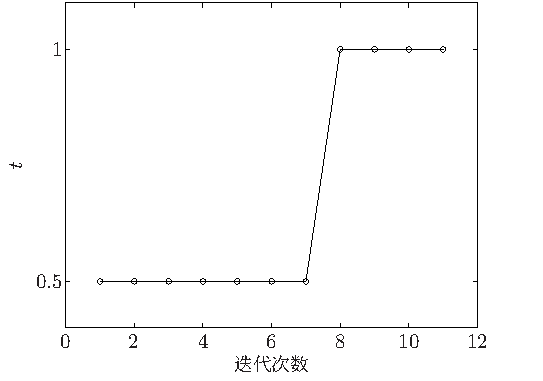
\includegraphics[width=.7\textwidth]{ch10-02.pdf}
\caption*{图10.2\quad 同一例题中步长随迭代次数的变化。第8次迭代取完整步，因此从第8次迭代开始可行。}
\end{figure}

% Source PDF page 558 (printed p. 544)
\begin{figure}[htbp]\centering
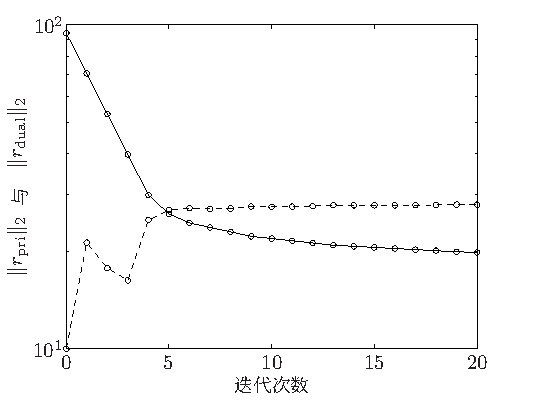
\includegraphics[width=.7\textwidth]{ch10-03.pdf}
\caption*{图10.3\quad 不可行初始点牛顿法求解具有100个变量、50个约束的等式约束解析中心问题的进展；该问题的 $\dom f=\R_{++}^{100}$ 与 $\{z\mid Az=b\}$ 不相交。图中给出 $\norm{r_{\rm pri}}_2$（实线）和 $\norm{r_{\rm dual}}_2$（虚线）。此时残差不收敛到零。}
\end{figure}
\begin{figure}[htbp]\centering
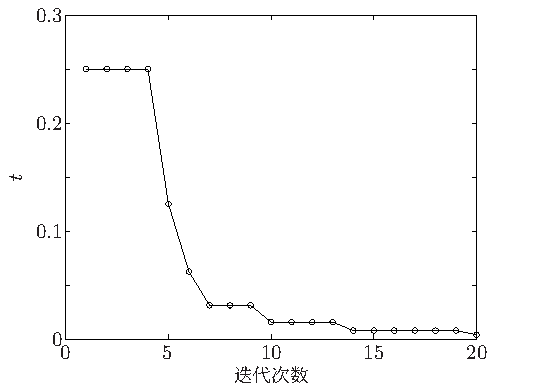
\includegraphics[width=.7\textwidth]{ch10-04.pdf}
\caption*{图10.4\quad 不可行例题中步长随迭代次数的变化。没有采用完整步，步长收敛到零。}
\end{figure}

% Source PDF page 559 (printed p. 545)
\begin{figure}[htbp]\centering
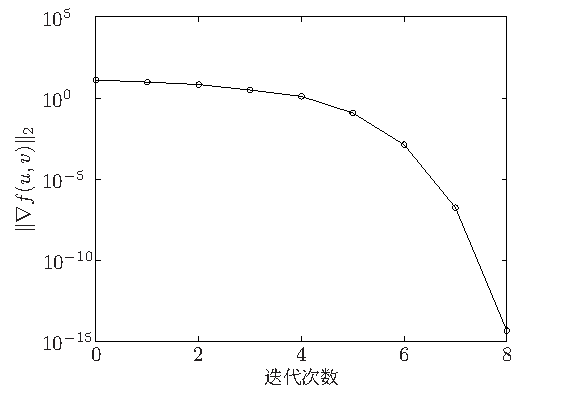
\includegraphics[width=.72\textwidth]{ch10-05.pdf}
\caption*{图10.5\quad 不可行初始点牛顿法求解凸凹博弈的进展。大约5次迭代后，二次收敛变得明显。}
\end{figure}
\begin{equation}\begin{bmatrix}H&A^\T\\A&0\end{bmatrix}\begin{bmatrix}v\\w\end{bmatrix}=-\begin{bmatrix}g\\h\end{bmatrix}.\tag{10.33}\end{equation}
假设 $H\in\mathbf S_+^n$，$A\in\R^{p\times n}$，且 $\rank A=p<n$。类似方法也可计算凸凹博弈的牛顿步，这时系数矩阵右下角分块是负半定的，见习题10.13。

\subsubsection*{求解完整 KKT 系统}
一种直接方法是求解整个 KKT 系统 (10.33)，即关于 $n+p$ 个变量的 $n+p$ 个线性方程。KKT 矩阵对称但不正定，因此适宜使用 $LDL^\T$ 分解，见第C.3.3节。如果不利用矩阵结构，代价为 $(1/3)(n+p)^3$ 次浮点运算。问题规模小，即 $n$、$p$ 不太大，或 $A$、$H$ 稀疏时，这可能是合理的方法。

\subsubsection*{通过消元求解 KKT 系统}
一种经常比直接求解完整 KKT 系统更好的方法，是消去变量 $v$，见第C.4节。先介绍最简单的 $H\succ0$ 的情况。由 KKT 方程
\[Hv+A^\T w=-g,\qquad Av=-h,\]
中的第一个方程解出 $v$：
\[v=-H^{-1}(g+A^\T w).\]

% Source PDF page 560 (printed p. 546)
代入第二个 KKT 方程，得到 $AH^{-1}(g+A^\T w)=h$，所以
\[w=(AH^{-1}A^\T)^{-1}(h-AH^{-1}g).\]
这些公式给出了计算 $v$ 和 $w$ 的方法。

$w$ 的表达式中出现的矩阵，是 $H$ 在 KKT 矩阵中的 Schur 补 $S$：
\[S=-AH^{-1}A^\T.\]
由于 KKT 矩阵的特殊结构，以及 $A$ 的秩为 $p$ 的假设，矩阵 $S$ 负定。

\begin{origalgorithm}{10.3}
\emph{用分块消元求解 KKT 系统。}

给定满足 $H\succ0$ 的 KKT 系统。
\begin{enumerate}
\item 形成 $H^{-1}A^\T$ 和 $H^{-1}g$。
\item 形成 Schur 补 $S=-AH^{-1}A^\T$。
\item 解 $Sw=AH^{-1}g-h$，得到 $w$。
\item 解 $Hv=-A^\T w-g$，得到 $v$。
\end{enumerate}
\end{origalgorithm}
第1步可通过 $H$ 的 Cholesky 分解，再进行 $p+1$ 次求解来完成，代价为 $f+(p+1)s$，其中 $f$ 是分解 $H$ 的代价，$s$ 是一次对应求解的代价。第2步需要一个 $p\times n$ 矩阵与 $n\times p$ 矩阵相乘。若不利用结构，代价为 $p^2n$ 次浮点运算；由于结果对称，只需计算 $S$ 的上三角部分。有时可以利用 $A$ 和 $H$ 的特殊结构，更高效地完成第2步。第3步可以对 $-S$ 作 Cholesky 分解；若不进一步利用 $S$ 的结构，代价为 $(1/3)p^3$。第4步可以使用第1步已计算的 $H$ 的分解，因此代价为 $2np+s$ 次浮点运算。假设在形成或分解 Schur 补时不利用结构，总浮点运算次数为
\[f+ps+p^2n+(1/3)p^3\]
（仅保留主项）。如果利用形成或分解 $S$ 时的结构，最后两项还会更小。

若 $H$ 可高效分解，分块消元的浮点运算次数就比用 $LDL^\T$ 分解直接求解 KKT 系统少。例如，若 $H$ 为对角矩阵，对应可分离目标函数，则 $f=0$、$s=n$，总代价为 $p^2n+(1/3)p^3$，仅随 $n$ 线性增长。若 $H$ 为带宽 $k\ll n$ 的带状矩阵，则 $f=nk^2$、$s=4nk$，总代价约为 $nk^2+4nkp+p^2n+(1/3)p^3$，仍仅随 $n$ 线性增长。$H$ 还可以有其他可利用的结构，如分块对角结构（对应分块可分离目标函数）、稀疏结构、对角加低秩结构；更多细节和例子见附录C与第9.7节。

\begin{origexample}{10.3}
\emph{等式约束解析中心。}考虑问题
\[\begin{array}{ll}\text{最小化}&-\displaystyle\sum_{i=1}^n\log x_i\\\text{约束条件}&Ax=b.\end{array}\]

% Source PDF page 561 (printed p. 547)
这里目标函数可分离，所以 $x$ 处的 Hessian 是对角矩阵：
\[H=\diag(x_1^{-2},\ldots,x_n^{-2}).\]
若用通用方法，如 KKT 矩阵的 $LDL^\T$ 分解计算牛顿方向，代价为 $(1/3)(n+p)^3$ 次浮点运算。

若用分块消元计算牛顿步，代价为 $np^2+(1/3)p^3$，比通用方法小得多。

事实上，这与第525页例10.2所述对偶问题中牛顿步的计算代价相同。对于该无约束对偶问题，Hessian 为
\[H_{\rm dual}=-ADA^\T,\]
其中 $D$ 是对角矩阵，$D_{ii}=(A^\T\nu)_i^{-2}$。形成该矩阵需要 $np^2$ 次浮点运算，对 $-H_{\rm dual}$ 作 Cholesky 分解来求牛顿步，需要 $(1/3)p^3$ 次浮点运算。
\end{origexample}

\begin{origexample}{10.4}
\emph{等式约束下的最短分段线性曲线。}考虑 $\R^2$ 中结点为 $(0,0),(1,x_1),\ldots,(n,x_n)$ 的分段线性曲线。为寻找满足等式约束 $Ax=b$ 的最短曲线，构造问题
\[\begin{array}{ll}\text{最小化}&(1+x_1^2)^{1/2}+\displaystyle\sum_{i=1}^{n-1}(1+(x_{i+1}-x_i)^2)^{1/2}\\\text{约束条件}&Ax=b,\end{array}\]
变量为 $x\in\R^n$，$A\in\R^{p\times n}$。目标为相邻变量对的函数之和，因此 Hessian $H$ 是三对角矩阵。用分块消元，可以约 $p^2n+(1/3)p^3$ 次浮点运算计算牛顿步。
\end{origexample}

\subsubsection*{$H$ 奇异时的消元}
上述分块消元法显然不适用于奇异 $H$，但只需简单修改，就可用于这一更一般情况。更一般的方法基于如下结果：KKT 矩阵非奇异，当且仅当对某个 $Q\succeq0$ 有 $H+A^\T QA\succ0$；此时对所有 $Q\succ0$ 都有 $H+A^\T QA\succ0$，见习题10.1。因此，例如，只要 KKT 矩阵非奇异，就有 $H+A^\T A\succ0$。

令 $Q\succeq0$ 为满足 $H+A^\T QA\succ0$ 的矩阵。KKT 系统 (10.33) 等价于
\[\begin{bmatrix}H+A^\T QA&A^\T\\A&0\end{bmatrix}\begin{bmatrix}v\\w\end{bmatrix}=-\begin{bmatrix}g+A^\T Qh\\h\end{bmatrix},\]
由于 $H+A^\T QA\succ0$，可以通过消元求解。

\subsection{例子}
本节给出一些较长的例子，说明怎样利用结构高效计算牛顿步，同时给出一些数值结果。

% Source PDF page 562 (printed p. 548)
\subsubsection*{等式约束解析中心}
考虑等式约束解析中心问题
\[\begin{array}{ll}\text{最小化}&f(x)=-\displaystyle\sum_{i=1}^n\log x_i\\\text{约束条件}&Ax=b.\end{array}\]
见例10.2和例10.3。对于 $p=100$、$n=500$ 的问题，比较三种方法。

第一种是带等式约束的牛顿法，第10.2节。牛顿步 $\Delta x_{\rm nt}$ 由 KKT 系统 (10.11) 定义：
\[\begin{bmatrix}H&A^\T\\A&0\end{bmatrix}\begin{bmatrix}\Delta x_{\rm nt}\\w\end{bmatrix}=\begin{bmatrix}-g\\0\end{bmatrix},\]
其中 $H=\diag(1/x_1^2,\ldots,1/x_n^2)$，$g=-(1/x_1,\ldots,1/x_n)$。如第546页例10.3解释的，可通过消元高效求解 KKT 系统，即求解
\[AH^{-1}A^\T w=-AH^{-1}g,\]
并令 $\Delta x_{\rm nt}=-H^{-1}(A^\T w+g)$。换言之，
\[\Delta x_{\rm nt}=-\diag(x)^2A^\T w+x,\]
其中 $w$ 为方程
\begin{equation}A\diag(x)^2A^\T w=b\tag{10.34}\end{equation}
的解。

图10.6给出误差随迭代次数的变化，不同曲线对应四个不同初始点。使用回溯参数 $\alpha=0.1$、$\beta=0.5$ 的线搜索。

第二种方法是对对偶问题使用牛顿法：
\[\text{最大化}\quad g(\nu)=-b^\T\nu+\sum_{i=1}^n\log(A^\T\nu)_i+n,\]
见第525页例10.2。这里通过求解
\begin{equation}A\diag(y)^2A^\T\Delta\nu_{\rm nt}=-b+Ay\tag{10.35}\end{equation}
得到牛顿步，其中 $y=(1/(A^\T\nu)_1,\ldots,1/(A^\T\nu)_n)$。比较 (10.35) 和 (10.34)，可见两种方法复杂度相同。图10.7给出四个不同初始点下的误差，回溯参数为 $\alpha=0.1$、$\beta=0.5$。

第三种是将第10.3节的不可行初始点牛顿法用于最优性条件
\[\nabla f(x^\star)+A^\T\nu^\star=0,\qquad Ax^\star=b.\]
牛顿步由求解
\[\begin{bmatrix}H&A^\T\\A&0\end{bmatrix}\begin{bmatrix}\Delta x_{\rm nt}\\\Delta\nu_{\rm nt}\end{bmatrix}=-\begin{bmatrix}g+A^\T\nu\\Ax-b\end{bmatrix}\]
得到。

% Source PDF page 563 (printed p. 549)
\begin{figure}[htbp]\centering
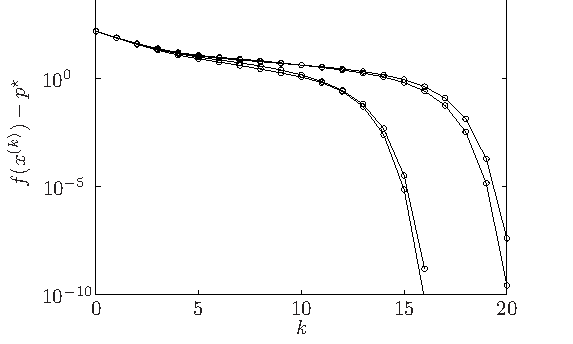
\includegraphics[width=.72\textwidth]{ch10-06.pdf}
\caption*{图10.6\quad 对大小为 $p=100$、$n=500$ 的等式约束解析中心问题使用牛顿法时的误差 $f(x^{(k)})-p^\star$。不同曲线对应四个不同初始点，最后的二次收敛清晰可见。}
\end{figure}
\begin{figure}[htbp]\centering
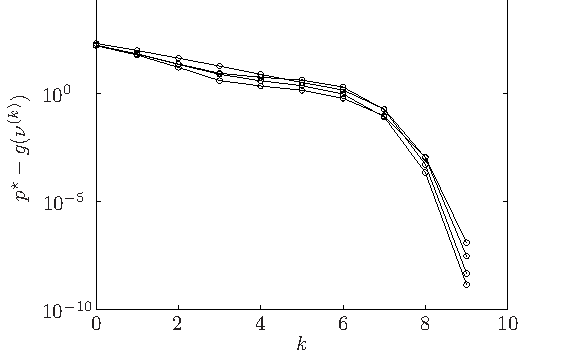
\includegraphics[width=.72\textwidth]{ch10-07.pdf}
\caption*{图10.7\quad 对等式约束解析中心问题的对偶使用牛顿法时的误差 $|g(\nu^{(k)})-p^\star|$。}
\end{figure}

% Source PDF page 564 (printed p. 550)
\begin{figure}[htbp]\centering
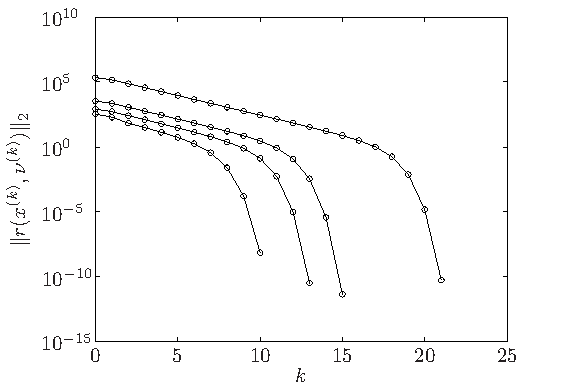
\includegraphics[width=.7\textwidth]{ch10-08.pdf}
\caption*{图10.8\quad 对等式约束解析中心问题使用不可行初始点牛顿法时的残差 $\norm{r(x^{(k)},\nu^{(k)})}_2$。}
\end{figure}
其中 $H=\diag(1/x_1^2,\ldots,1/x_n^2)$，$g=-(1/x_1,\ldots,1/x_n)$。这个 KKT 系统同样可以通过消元高效求解，代价与 (10.34) 或 (10.35) 相同。例如，先求解
\[A\diag(x)^2A^\T w=2Ax-b,\]
再由
\[\Delta\nu_{\rm nt}=w-\nu,\qquad\Delta x_{\rm nt}=x-\diag(x)^2A^\T w\]
得到 $\Delta\nu_{\rm nt}$ 与 $\Delta x_{\rm nt}$。图10.8给出四个不同初始点下残差
\[r(x,\nu)=(\nabla f(x)+A^\T\nu,Ax-b)\]
范数随迭代次数的变化，回溯参数为 $\alpha=0.1$、$\beta=0.5$。

图中可见，对这个问题，对偶方法似乎更快，但只快两三倍。它约经6次迭代进入二次收敛区域，而原始方法需12至15次，不可行初始点牛顿法需10至20次。

这些方法的初始化要求也不同。原始方法需要一个已知原始可行点，即满足 $Ax^{(0)}=b$、$x^{(0)}\succ0$。对偶方法需要一个对偶可行点，即 $A^\T\nu^{(0)}\succ0$。依具体问题不同，二者之一可能更容易获得。不可行初始点牛顿法不需要这样的初始化，唯一要求是 $x^{(0)}\succ0$。

\subsubsection*{最优网络流}
考虑具有 $n$ 条边、$p+1$ 个结点的连通有向图或网络。用 $x_j$ 表示弧 $j$ 上的流量或交通量，$x_j>0$ 表示沿弧方向流动。
